To numerically solve a set of PDEs, iterative methods (finite difference, finite volume or finite element methods) are frequently used to approximate the solution through a discretized (step by step) phenomena. Thus, the continuous time and space domains are discretized so that a set of numerical computations are iteratively (time discretization) applied onto a mesh (space discretization). In other words, the PDEs are transformed to a set of numerical computations applied at each time step on elements of the discretized space domain. Among those numerical computations is found a set of numerical schemes, also called \textit{stencil computations}, and a set of auxiliary computations also needed to perform the simulation, and also called \emph{local computations}.
This section gives formal definitions of what we call a \textit{stencil program} and its computations. Then, the different mid-grain parallelization techniques which can be applied on such program, are presented.

%-------------------------------------
\subsection{Time, mesh and data}

$\Omega=\mathbb{R}^n$ is the continuous space domain of a numerical simulation. %For example, if $n=3$, any geographic point on earth could be represented in this space in a given geographic coordinate system.
A mesh $\mathcal{M}$ defines the discretization of the continuous space domain $\Omega$ of a set of PDEs and is defined as follows.

\begin{mydef}
\textit{A mesh is a connected undirected graph $\mathcal{M}=(V,E)$, where $V\subset \Omega$ is the set of vertices and $E\subseteq V^2$ the set of edges. The set of edges $E$ of a mesh $\mathcal{M}=(V,E)$ does not contain bridges. It is said that the mesh is applied onto $\Omega$}.
\end{mydef}
\begin{figure}[!h]\begin{center}
  \resizebox{8cm}{!}{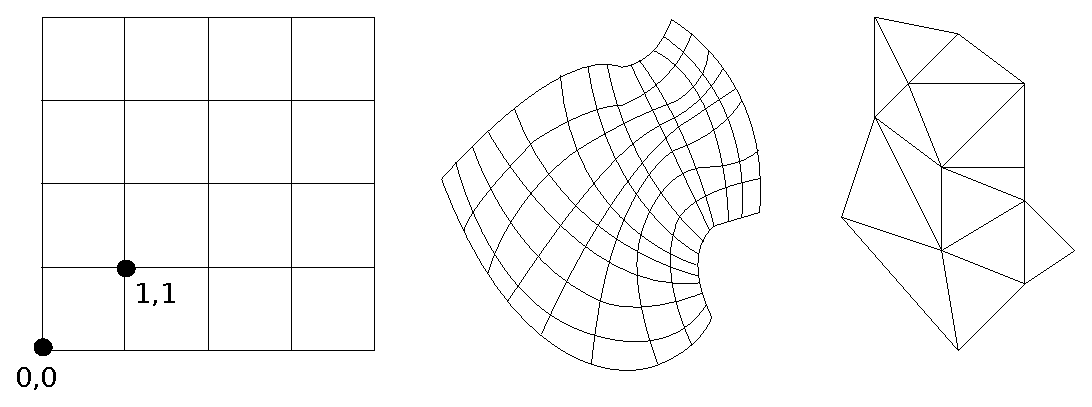
\includegraphics{./images/maillages.pdf}}
  \caption{From left to right, Cartesian, curvilinear and unstructured meshes.}
  \label{fig:mesh}
\end{center}\end{figure}
\begin{mydef}
\textit{The dimension of a mesh $\mathcal{M}=(V,E)$ applied onto $\Omega=\mathbb{R}^n$ is denoted $dim(\mathcal{M})=n$.}
\end{mydef}
A mesh can be structured (as Cartesian or curvilinear meshes), unstructured, regular or irregular (without the same topology for each element) and hybrid as illustrated in Figure~\ref{fig:mesh}.

\medskip
\noindent \textbf{Definitions}
%\begin{mydef}
\begin{itemize}
\item \textit{An entity $e$ of a mesh $\mathcal{M}=(V,E)$ is defined as a subset of its vertices and edges, $e\subset (V\cup E)$.
\item A mesh entities group is denoted $E$ such that $E \in \mathcal{P}(V\cup E)$. It represents a set of entities of the same type.
\item Finally the set of mesh entities groups of a simulation is denoted $\mathcal{E}$.}
\end{itemize}
%\end{mydef}

For example, in a 2D Cartesian mesh an entity could be a cell, made of four vertices and four edges, or simply a vertex. As a result a group of cells and a group of vertices could be defined in $\mathcal{E}$. %This type can be defined as the sets containing exactly four vertices and four edges connected as a cycle. Another type of entities simply are the vertices ($V$) and can be defined as all singletons formed of a single vertex of $V$.

\medskip
This covers the space discretization, however there is also the time dimension which has to be discretized in the simulation.

\medskip
\noindent \textbf{Definitions}
%\begin{mydef}
\begin{itemize}
\item \textit{We denote a scalar as an identifier associated to a numerical value and applied onto a mesh $\mathcal{M}$ where $dim(\mathcal{M})=0$. In other words a scalar can be seen as a variable containing a numerical value. The set of scalars is denoted $\mathcal{S}$.}
\item \textit{$\mathcal{T}=\mathbb{R}$ is the continuous time domain of a numerical simulation.}
\item \textit{The discretization of the continuous time domain $\mathcal{T}$ is denoted as the pair $T(\Delta t,conv)$.} 
\begin{itemize}
\item \textit{$\Delta t \in \mathcal{S}$ represents the time interval of the numerical simulation, such that for a current time iteration $t_i$, the next time iteration is $t_{i+1} = t_i + \Delta t$. The default value of $\Delta t$ is $1$.
\item $conv:\mathcal{S}^n \rightarrow bool$ is a function which returns a boolean from a set of scalar variables. This function represents the convergence criteria of the simulation. 
\item At a given time step, the convergence criteria is evaluated such that if $conv$ returns $true$ the next time step can start such that $t_{i+1} = t_i + \Delta t$, otherwise the simulation ends. For example, the simplest $conv$ is typically to have two scalars: $t$ the time, and a fix number of iterations denoted $it$. At each time step $\Delta t=1$, and $conv$ returns the boolean expression $t<it$.}
\end{itemize}
\end{itemize}
%\end{mydef}

%$T$ is responsible for the iteration time steps of the numerical simulation. A numerical simulation though does not run forever and must be stopped at some point. Some simulations choose a fix number of time iteration, others compute a \emph{convergence} criteria at the end of each time iteration to determine if the simulation has to continue. A convergence criteria is computed by a reduction computation that will be detailed in the next section.

In a numerical simulation, as a set of scalars can be applied onto a mesh with a nil dimension, a set of data elements, or quantities, can be applied onto meshes of dimension superior or equal to zero. Those quantities represent, as well as scalars, the set of values to compute, or to use, for computations.

\noindent \textbf{Definitions}
%\begin{mydef}
\begin{itemize}
\item \textit{A quantity is a function $\delta: E_{\delta} \mapsto V_{\delta}$ which associates each entity of a group $e\in E_{\delta}$ to a value $v\in V_{\delta}$ where $V_{\delta}$ is a data type, typically $\mathbb{R}$, $\mathbb{N}$ or $\mathbb{C}$.
\item The set of quantities applied onto the mesh is denoted $\Delta$.
\item In the rest of this paper, the group of mesh entities on which a quantity $\delta$ is mapped is denoted $entity(\delta)=E_{\delta}$.}
\end{itemize}
%\end{mydef}

Another option, closer to the applied mathematics domain, would have been to define $\delta$ as the function over $E_{\delta} \times T$; however the approach chosen for now in this work is to let the user be aware of the number of data he is using and what exactly for.

%-----------------------
\subsection{Computations}

In this section are considered two different types of computations, a reduction or a numerical kernel. 

\noindent \textbf{Definitions}
%\begin{mydef}
\begin{itemize}
\item \textit{A computation domain $D$ is a subpart  a mesh entities group, $D \subset E \in \mathcal{E}$.
\item The set of computation domains of a numerical simulation is denoted $\mathcal{D}$.
\item A neighborhood $n$ is a function which for a given entity $e \in E_i$, returns a set of $m$ entities in $E_j$, $n : E_i \rightarrow E_j^m$. One can notice that $i = j$ is possible.
\item The set of neihborhood functions in a numerical simulation is denoted $\mathcal{N}$.
\item A single data is written during a computation and is denoted $w \in \Delta$. Thus, the computation domain of the computation is $D \subset E_w=entity(w)$.
\item A set of data to read and use in a computation is denoted $R$. Each element of $R$ is a tuple $(r,n)$, where $r \in \Delta$ and $n$ is a neighborhood function such that $n : E_w \rightarrow entity(r)^m$. The neighborhood indicates which entities, on which $r$ is applied, will be read during the computation.
\item A numerical expression $\text{exp}_{w}: entity(w) \times R^n \rightarrow V_{w}$ is a function that computes the value of the written quantity $w \in \Delta$ for a given entity $e \in entity(w)=E_w$, using a set of input data $R$.
\item A computation kernel $k$ of a numerical simulation is defined as $k(R,w,\text{exp},D)$, where $R$ is the set of data read, $w \in \Delta$ is the unique data written, $\text{exp}$ is a numerical expression, and $D \in \mathcal{D}$ is the computation domain.}
\end{itemize}
%\end{mydef}
%If the number of computations in $\Gamma$ is $card(\Gamma)=n$, such that $\bigcup_{i=0}^{n-1}c_i = \Gamma$, then $\bigcup_{i=0}^{m-1}R_i \cup w_i \subseteq \Delta$.

Most of the time we can dissociate two types of kernel computations.

\noindent \textbf{Definitions}
%\begin{mydef}
\begin{itemize}
\item \textit{We denote by $identity$ the identity function $x=x$.
\item A kernel computation $k(R,w,\text{exp},D) \in \Gamma$ is a stencil kernel $\iff \exists (r,n) \in R$ such that $n \neq identity$.
\item A kernel computation $k(R,w,\text{exp},D) \in \Gamma$ is a local kernel $\iff \forall (r,n) \in R$, $n = identity$.}
\end{itemize}

\noindent \textbf{Property}
\textit{A kernel for which all data read and written are applied onto a mesh of dimension $0$ is a local kernel.}

A reduction computation is a computation which takes data applied onto meshes and returns a data with a dimension reduced to zero, in other words a scalar. A reduction is typically used to compute the convergence criteria of the time loop of the simulation. Occasionally reductions can also be performed during a time iteration. %This last usage is typically done to have a conditionnal branch to choose one computation or another, or to compute a dynamic time step for example.

\medskip
\noindent \textbf{Definitions}
%\begin{mydef}
\begin{itemize}
\item \textit{A reduction computation $r$ of a numerical simulation is defined as $r(R,w,red)$, where $R$ is the set of data read, $w \in \mathcal{S}$ is the scalar written, and $\text{red}$ is an associative reduction function.
% \item For any $i,j$ such that $r_i \in R$ and $r_j \in R$, if $dim(mesh(r_i))=dim(mesh(r_j))=n$.
% \item The data written by the reduction $w$ verifies $dim(mesh(w))<n$.
\item A reduction function $\text{red}: \Delta^n \rightarrow \mathcal{S}$ is an operation which reduces a set of data in $\Delta$ (on it sentities) to a single scalar variable in $\mathcal{S}$. The reduction function must be associative.
\item The set of $n$ ordered computations (kernel or reduction) of a numerical simulation is denoted $\Gamma = [c_i]_{0 \leq i \leq n-1}$, such that $\forall c_i,c_j \in \Gamma$, if $i \leq j$, then $c_i$ is computed before $c_j$.
\item Finally, a \textit{multi-stencil program} is defined by the septuplet $\mathcal{MSP}(T,\mathcal{M},\mathcal{E},\mathcal{D},\Delta, \mathcal{S},\Gamma)$.}
\end{itemize}
%!!!!!!!  est-ce qu'on fusionne le maillage, les entites et les domaines ?????
%\end{mydef}


For example, in Figure~\ref{fig:ex1}, assuming that the computation domain (full lines) is denoted $dc1$ and the stencil shape is $n1$, the stencil kernel can be defined as:
\begin{equation*}
R: \{(B,n1)\}, \quad w: A, \quad d: dc1,
\end{equation*}
\begin{equation*}
exp: A(x,y)=B(x+1,y)+B(x-1,y)+B(x,y+1)+B(x,y-1).
\end{equation*}
On the other hand, in the example of Figure~\ref{fig:ex2}, assuming the computation domain is $dc2$ and the stencil shape is $n2$, the stencil kernel is defined as:
\begin{equation*}
R: \{(C,n2),(A,identity)\}, \quad w: A, \quad d: dc2,
\end{equation*}
\begin{equation*}
exp: A(x,y)=A(x,y)+C(x1,y1)+C(x1+1,y1).
\end{equation*}

\begin{figure}
\begin{center}
\subfloat[Mesh and mesh domains.\label{fig:meshbase}]{
\resizebox{8cm}{!}{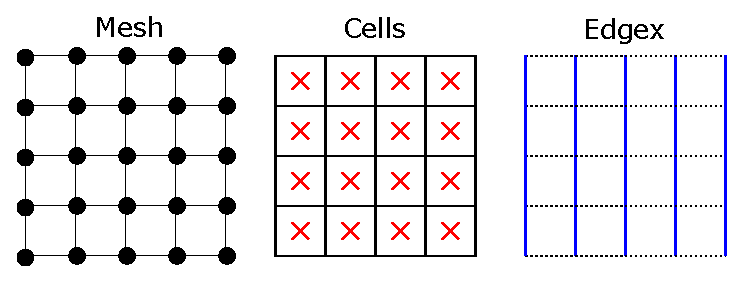
\includegraphics{./images/mesh.pdf}}
}\\
\hspace{10pt}
\subfloat[4-neighborhood stencil.\label{fig:ex1}]{
\resizebox{5cm}{!}{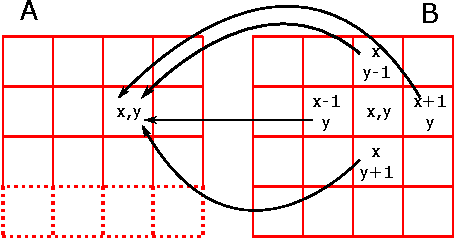
\includegraphics{./images/stencil1.pdf}}
}
\vspace{20pt}
\subfloat[4-neighborhood stencil.\label{fig:ex2}]{
\resizebox{5cm}{!}{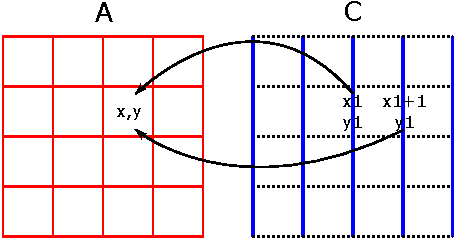
\includegraphics{./images/stencil2.pdf}}
}
\end{center}
\caption{(a) a Cartesian mesh and two kind of mesh entities, (b) an example of stencil kernel on cells, (c) an example of stencil kernel on two different entities of the mesh.}
\label{fig:gspmsp}
\end{figure}

A stencil program has been formally defined in this section. This formalism is used in the next Section to define two mid-grain parallelization techniques of a multi-stencil program.


